\documentclass[aps,prd,twocolumn,superscriptaddress,nofootinbib,longbibliography,floatfix]{revtex4-2}
\usepackage{amsmath,amssymb,bm,mathtools}
\usepackage{graphicx}
\usepackage{booktabs}
\usepackage{hyperref}
\usepackage{siunitx}
\usepackage{physics}
\usepackage{microtype}
\usepackage{enumitem}
\hypersetup{hidelinks}

\newcommand{\Y}{\mathcal{Y}}
\newcommand{\Q}{\mathcal{Q}}
\newcommand{\FT}{\mathcal{F}_{T}}
\newcommand{\Ffull}{\mathcal{F}}
\newcommand{\LCDM}{\Lambda\mathrm{CDM}}
\newcommand{\mpl}{M_{\rm Pl}}

\begin{document}

\title{A Stable Single-Metric Relativistic Modified-Gravity Cosmology without Particle Cold Dark Matter or a Bare Cosmological Constant}

\author{Panagiotis Karmiris}
\email{unbinder@msn.com}
\affiliation{Independent Researcher, Greece}

\date{September 2, 2026}

\begin{abstract}
We construct and test a single-metric relativistic modified-gravity cosmology in which the particle cold-dark-matter density and the bare cosmological constant are set to zero. The theory combines an aether scalar--tensor sector with a Type-II minimally modified gravity constraint sector governing late-time acceleration. In the scalar--vector sector, the kinetic function is nonseparable, $\Ffull(\Y,\Q)=\FT(\Q)+\Y\Gamma(\Q)+J(\Y)$, with $\Gamma(\Q)$ fixed by the conserved homogeneous scalar current rather than introduced as a new fitted function. The mixed interaction vanishes on the homogeneous FLRW background and at the screened static point $\Q=\Q_0$, while converting the radiation-era scalar characteristic polynomial into a strictly Hurwitz form on the physical branch. The acceleration sector is auxiliary at the perturbative level and adds no new propagating scalar degree of freedom. We derive the scalar perturbation mapping implemented in CLASS and show that the direct scalar source contains an exact $K_Q-\Q F_{,\Y}=0$ cancellation. A nonlinear Hamiltonian analysis gives six physical degrees of freedom in the analyzed phase-space formulation. The propagating scalar has a minimum canonically normalized cubic derivative cutoff $\Lambda_{\rm sc}=1.4742\times10^{-6}\,{\rm eV}$ over the tested cosmological branch; the companion first-order scalar is governed by a nondegenerate second-class Dirac pair with an infrared-finite and ultraviolet-soft inverse. A fresh six-likelihood evaluation using Planck 2018 temperature and polarization data and lensing, DESI DR2 BAO, and Pantheon+ gives $\chi^2=2422.69597$, compared with $2428.9192$ for the matched optimized $\LCDM$ reference. For the stated parameter-count convention, $\Delta{\rm AIC}=-4.223$ and $\Delta{\rm BIC}=+1.557$. An independent profile in particle CDM places the exact zero-CDM realization at $\Delta\chi^2=0.958$ from the sampled profile minimum. Thus the tested data do not require a particle cold-dark-matter component, although they do not uniquely select zero particle CDM. The same scalar function retains the tested no-halo galactic limit because the new mixed operator vanishes in the relevant static screened configuration.
\end{abstract}

\maketitle

\section{Introduction}\label{sec:intro}
The standard cosmological model explains a wide range of observations through general relativity supplemented by cold dark matter (CDM) and a cosmological constant. Its empirical success is substantial, particularly for the cosmic microwave background (CMB), baryon acoustic oscillations (BAO), gravitational lensing, and large-scale structure \cite{Planck2020VI,DESI2024VI,DESIDR2II2025,Madhavacheril2024,DESY3Cosmology2022}. At galactic scales, the tight relation between baryonic distributions and observed accelerations has motivated the modified Newtonian dynamics (MOND) program and relativistic attempts to reproduce its phenomenology \cite{Milgrom1983,Bekenstein2004,LelliMcGaughSchombert2016,McGaughLelliSchombert2016}. A central theoretical challenge is to retain the empirical galactic regularities while obtaining a viable relativistic theory with stable perturbations and a cosmological component capable of replacing the dynamical role normally assigned to particle CDM. This question is especially timely because contemporary expansion-history and structure analyses continue to sharpen tests of departures from the baseline model \cite{DiValentino2021,Schoneberg2022,PerivolaropoulosSkara2022,DES2024SN,EuclidWeakLensing2024}.

Aether scalar--tensor (AeST) gravity provides a single-metric setting containing a metric, a unit timelike vector, and a shift-symmetric scalar \cite{SkordisZlosnik2021,SkordisZlosnik2022}. Subsequent studies have examined its nonlinear Hamiltonian structure, cosmological dynamics, quasistatic spherical solutions, galaxy-cluster configurations, and compact stars \cite{BatakiSkordisZlosnik2024,RosaZlosnik2024,VerwayenSkordisBoehm2024,DurakovicSkordis2024,ReyesSakstein2024,ReyesSakstein2025}. These results motivate a direct test of whether a carefully specified scalar--vector sector can act as an effective cold component without introducing particle dark matter.

Late-time acceleration is treated here through the auxiliary constraint sector of VCDM, a Type-II minimally modified gravity construction whose cosmological applications and perturbative degree-of-freedom structure have been studied independently \cite{DeFeliceMukohyamaPookkillath2021,DeFeliceMaedaMukohyamaPookkillath2022,GanzMartensMukohyamaNamba2023,AkarsuEtAl2024VCDM,AkarsuEtAl2026VCDM}. This sector changes the homogeneous gravitational dynamics without adding an additional propagating scalar mode. Combining it with AeST allows the particle-CDM density and bare cosmological constant to be fixed to zero while retaining independent control of the effective cold and acceleration sectors.

The new theoretical result of this work concerns the scalar kinetic structure. A free function separable between timelike and spacelike scalar invariants admits a radiation-era slow mode that is not strictly damped on the physical early-time solution. We show that the minimal nonseparable operator $\Y\Gamma(\Q)$ removes this defect when $\Gamma$ is fixed by the already existing conserved scalar current. The construction therefore introduces no new field, no new free function, and no additional continuous fit parameter. On FLRW, $\Y=0$, so the calibrated homogeneous scalar background is unchanged; in the screened static configuration, $\Q=\Q_0$ and $\Gamma(\Q_0)=0$, so the galactic function is unchanged.

We carry this construction through a full theory-to-data validation. We derive the perturbation equations and their map into CLASS \cite{Lesgourgues2011CLASS,Blas2011CLASS}, audit the combined nonlinear constraint algebra, canonically normalize the cubic scalar interactions, compare the nonseparable theory against its separable control at fixed background, and only then optimize the frozen numerical theory against Planck 2018, DESI DR2, and Pantheon+ likelihoods \cite{Brout2022,Scolnic2022,DESIDR2II2025}. A separate profile in an explicit particle-CDM density tests whether the data require such a component once the effective AeST cold density is allowed to readjust independently.

The claims of this article are deliberately limited to the classical relativistic theory, its linear cosmology, the tested static galactic limit, and the stated effective-field-theory domain. We do not infer a fundamental quantum ultraviolet completion from the classical cutoff analysis, and we do not interpret a raw non-nested likelihood difference as a Gaussian discovery significance.

\section{Single-metric relativistic theory}\label{sec:theory}
\subsection{Aether scalar--tensor sector}
Ordinary matter couples minimally and universally to one physical metric $g_{\mu\nu}$. Let $A^\mu$ be a unit timelike vector, $A^\mu A_\mu=-1$, and $\phi$ a shift-symmetric scalar. Define
\begin{align}
F_{\mu\nu}&=2\nabla_{[\mu}A_{\nu]},&
J^\mu&=A^\nu\nabla_\nu A^\mu,\\
q_{\mu\nu}&=g_{\mu\nu}+A_\mu A_\nu,&
\Q&=A^\mu\nabla_\mu\phi,\\
\Y&=q^{\mu\nu}\nabla_\mu\phi\nabla_\nu\phi.
\end{align}
The covariant scalar--vector sector is the AeST action \cite{SkordisZlosnik2021,SkordisZlosnik2022,BatakiSkordisZlosnik2024}, with bare cosmological constant fixed to zero,
\begin{widetext}
\begin{align}
S_{\rm AeST}=&\frac{1}{16\pi\widetilde G}\int d^4x\sqrt{-g}\Big\{R-\frac{K_B}{2}F_{\mu\nu}F^{\mu\nu}
 +(2-K_B)\left(2J^\mu\nabla_\mu\phi-\Y\right)
-\Ffull(\Y,\Q)-\lambda(A^\mu A_\mu+1)\Big\}
+S_m[g_{\mu\nu},\psi_m].
\label{eq:aest-action}
\end{align}
\end{widetext}
No disformal matter metric is introduced.

\subsection{Nonseparable scalar kinetic function}
The scalar free function is
\begin{equation}
\Ffull(\Y,\Q)=\FT(\Q)+\Y\Gamma(\Q)+J(\Y),
\label{eq:fullF}
\end{equation}
where
\begin{equation}
\FT(\Q)=-4K_2Z_0^2\left[\cosh\left(\frac{\Q-\Q_0}{Z_0}\right)-1\right],
\label{eq:FT}
\end{equation}
\begin{equation}
\Gamma(\Q)=\frac{2K_2Z_0}{\Q}\sinh\left(\frac{\Q-\Q_0}{Z_0}\right),
\label{eq:Gamma}
\end{equation}
and the static galactic function is
\begin{align}
J(\Y)=&\frac{a_0^2(2-K_B)}{\beta_0^3}\Bigg[-\frac{2\sqrt{\Y}\beta_0(\beta_0+1)}{a_0}
+\frac{\Y\beta_0^2}{a_0^2}\nonumber\\
&+2(\beta_0+1)^2\ln\left(1+\frac{\sqrt{\Y}\beta_0}{a_0(\beta_0+1)}\right)\Bigg].
\label{eq:JY}
\end{align}
The relevant temporal derivatives are
\begin{align}
\mathcal{F}_{T,\Q}&=-4K_2Z_0\sinh\left(\frac{\Q-\Q_0}{Z_0}\right),\\
\mathcal{F}_{T,\Q\Q}&=-4K_2\cosh\left(\frac{\Q-\Q_0}{Z_0}\right),\\
\mathcal{F}_{T,\Q\Q\Q}&=-\frac{4K_2}{Z_0}\sinh\left(\frac{\Q-\Q_0}{Z_0}\right),
\end{align}
and
\begin{align}
\Gamma_{,\Q}=\frac{2K_2}{\Q^2}\Bigg\{&\Q\cosh\left(\frac{\Q-\Q_0}{Z_0}\right)\nonumber\\
&-Z_0\sinh\left(\frac{\Q-\Q_0}{Z_0}\right)\Bigg\}.
\label{eq:GammaQ}
\end{align}
The essential minimality property is that $\Gamma$ is fixed by the homogeneous current, not independently fitted. Removing the mixed term provides a separable control theory; no additional field or continuous parameter is required to pass from that control to Eq.~\eqref{eq:fullF}.

\subsection{Auxiliary acceleration sector}
Late-time acceleration is supplied by a Type-II minimally modified gravity sector of the VCDM class \cite{DeFeliceMukohyamaPookkillath2021,DeFeliceMaedaMukohyamaPookkillath2022,GanzMartensMukohyamaNamba2023,AkarsuEtAl2024VCDM}. In ADM variables, the part relevant for the auxiliary scalar $\varphi_V$ and its constraint multiplier can be written, up to the standard Einstein--Hilbert ADM contribution and gauge-fixing term, as
\begin{align}
S_V=\mpl^2\!\int dt\,d^3x\,N\sqrt{\gamma}\Big[&-V(\varphi_V)-\frac34\lambda_C^2\nonumber\\
&-\lambda_C(K+\varphi_V)-\mathcal L_{\rm gf}\Big].
\label{eq:vcdm-aux}
\end{align}
Varying $\lambda_C$ gives
\begin{equation}
\lambda_C=-\frac23(K+\varphi_V),
\end{equation}
so the reduced deformation is
\begin{equation}
\mathcal L_{V,\rm red}=\mpl^2\left[\frac{(K+\varphi_V)^2}{3}-V(\varphi_V)-\mathcal L_{\rm gf}\right].
\label{eq:vcdm-red}
\end{equation}
For generic scalar perturbations with $k\neq0$, the auxiliary equations enforce $\delta\varphi_V=0$ together with the corresponding multiplier constraints; after Schur elimination this sector adds no propagating scalar degree of freedom. This is the key reason it can alter the background acceleration history without introducing a dark-energy fluid or an extra scalar wave mode \cite{DeFeliceMaedaMukohyamaPookkillath2022}.

In the numerical background parameterization, the reconstructed acceleration history is represented by a fourth-order basis with coefficients $s_1,\ldots,s_4$ and present closure density $\Omega_{V}$. Flat closure is recomputed at every likelihood point,
\begin{equation}
\Omega_V=1-\frac{\omega_b+\omega_{\rm aest}+\omega_r}{h^2},
\label{eq:vcdm-closure}
\end{equation}
for the zero-particle-CDM realization, while one dependent polynomial coefficient is fixed by the basis normalization. The final fit varies only one independent shape coefficient, $s_4$, from this acceleration sector.

\subsection{Regime separation}
The construction assigns distinct roles to distinct operators. The temporal scalar sector determines the homogeneous effective cold component; $J(\Y)$ determines the quasistatic MOND response; the mixed-current operator controls the radiation-era scalar gradient structure; and the auxiliary Type-II constraint sector supplies the reconstructed late-time acceleration. This separation is used throughout the validation to avoid attributing a successful observable to an unnecessarily complicated sector.

\section{Methodology and validation protocol}\label{sec:methods}
A central methodological choice was to separate theory construction from statistical optimization. The scalar kinetic structure, constraint analysis, perturbation equations, and stability conditions were fixed before the final likelihood parameters were optimized. The numerical source used for the final fit was then frozen by SHA-256, so likelihood improvement could not feed back into the field equations.

\subsection{Analytic background and current checks}
The FLRW scalar current was derived directly from the action and the exact closed-form solution for $\Q(a)$ was checked symbolically and numerically. The nonseparable and separable-control implementations were required to agree at the homogeneous scalar-background level because $\Y=0$ on FLRW. The particle-CDM density, bare cosmological constant, and auxiliary dark-energy-fluid density were fixed to zero in the final realization.

\subsection{Quadratic perturbation derivation}
The mixed operator was expanded to quadratic order about FLRW before any CLASS source change was made. The derivation was performed first in field variables and then mapped to the physical scalar combination $\chi$ used by the solver. A separate order-counting check established that $F_{,\Y\Q}$ first contributes as a cubic interaction rather than a new direct quadratic source. The exact identity $K_Q=\Q F_{,\Y}$ was imposed analytically in the final evolution equation; it was not evaluated by subtracting two nearly equal floating-point quantities at early times.

\subsection{Constraint and stability analysis}
The combined gravity/scalar/vector/auxiliary system was analyzed with a Dirac--Bergmann constraint classification. First-class null directions and the rank of the second-class block were checked independently. The Type-II acceleration sector was also reduced by explicit elimination of its auxiliary variables, confirming that it contributes no additional propagating scalar mode. The nonseparable scalar operator adds neither a configuration field nor a higher-time-derivative term.

The radiation-era reduced system was required to have a strictly Hurwitz characteristic polynomial on the physical branch. Separately, the propagating scalar was canonically normalized through cubic order, including the temporal, mixed, and MOND vertices. The remaining first-order scalar was treated through its reduced symplectic/Dirac structure, not by assigning it an artificial second-order kinetic eigenvalue.

\subsection{Boltzmann-code implementation and numerical regression}
The derived equations were implemented in CLASS \cite{Lesgourgues2011CLASS,Blas2011CLASS}. A matched control implementation differed only by removal of the nonseparable mixed-current contribution in the direct scalar source. Both implementations used identical homogeneous parameters, initial conditions, compilation settings, and output requests. The complete theory was required to produce finite bounded internal histories, finite CMB spectra through $\ell=2500$, finite positive linear matter spectra over the tested range, and the expected horizon-crossing behavior before likelihood evaluation.

The matched operator-removal test is an ablation, not a second phenomenological model fit. Its purpose is causal: it quantifies the response produced by the nonseparable operator while keeping the background fixed. This also checks that the operator is not observationally inert or merely a background reparameterization.

\subsection{Likelihoods and optimization}
The final likelihood stack consists of Planck 2018 high-$\ell$ TTTEEE-lite, Planck low-$\ell$ TT, Planck low-$\ell$ EE, Planck lensing, DESI DR2 BAO \cite{DESIDR2II2025}, and Pantheon+ supernovae \cite{Brout2022,Scolnic2022}. Likelihood evaluation used Cobaya \cite{TorradoLewis2021} in a frozen Python environment with NumPy 1.26.4 and a fixed external-likelihood package tree.

Seven coordinates were optimized,
\begin{equation}
\{H_0,\omega_b,\omega_{\rm aest},s_4,n_s,\ln(10^{10}A_s),\tau_{\rm reio}\}.
\end{equation}
At every trial point, flat closure $\Omega_V$ and the dependent acceleration-basis coefficient were recomputed rather than held at values inherited from the initial point. The exact best INI file was independently replayed, tested for evaluator-label invariance, locally polished, and subjected to symmetric positive/negative coordinate displacements. This provided a local stationarity certificate after the initial simplex optimizer reached its function-evaluation ceiling.

\subsection{Independent particle-CDM profile}
To distinguish a theoretically imposed zero-CDM realization from a data-driven preference, a separate analysis promoted $\omega_{\rm cdm}$ to a profile coordinate. At each fixed $\omega_{\rm cdm}$ value, $\omega_{\rm aest}$ and the cosmological fit coordinates were reoptimized independently. The conclusion drawn from this profile is deliberately limited: it tests whether a nonzero particle-CDM density is required by the selected likelihoods, not whether the observations uniquely select $\omega_{\rm cdm}=0$.

\subsection{Galactic validation and provenance}
The static galactic test uses the same $J(\Y)$ function as the cosmological theory. Because $\Gamma(\Q_0)=0$ in the screened static configuration, the nonseparable operator does not alter that test. The retained galaxy sample contains 132 SPARC systems and 2654 rotation-curve points, with no fitted particle-dark-matter halo parameters. The publication archive stores the machine-readable summary and provenance of this calculation rather than rerunning it during manuscript compilation \cite{LelliMcGaughSchombert2016}.

\subsection{AI-assisted research workflow and human verification}
Substantive AI assistance was used during parts of the research workflow. OpenAI ChatGPT (GPT-5.6 Sol) and Google Antigravity using Gemini 3.7 Flash (High reasoning) assisted with algebraic cross-checking, code generation and debugging, workflow organization, literature organization, and manuscript drafting. AI output was never treated as numerical evidence by itself: executable calculations were run in the author's local environments; proposed source changes were inspected before acceptance; analytic identities were checked symbolically or against independent numerical evaluations; final likelihood totals were replayed from frozen parameter files; and publication claims were checked against the retained source-of-truth artifacts and cited literature. The author performed the final scientific review and assumes responsibility for the calculations and conclusions.

\subsection{Reproducibility discipline}
Transient compiler trees and exploratory intermediate files were excluded from the public release. The retained publication record consists of source-of-truth equations, the exact optimized parameter file, machine-readable results, source hashes, figure-generation code, environment information, and regression scripts. The final CLASS perturbation source is identified by a cryptographic hash given in Appendix~\ref{app:repro}. This separation keeps the public repository testable without requiring readers to understand the internal development history.

\section{Results}\label{sec:results}
\subsection{Radiation-era stability}
The scalar radiation-sector characteristic polynomial is
\begin{equation}
A\lambda^2+B\lambda+C=0,
\end{equation}
with
\begin{align}
A&=\frac{2I_0K_B}{\Q a^3}-4K_B+8,\\
B&=HA,\\
C&=\frac{2HI_0(2-K_B)}{a^3}.
\end{align}
On the expanding physical branch $H>0$, $I_0>0$, $\Q>0$, $a>0$, and $0<K_B<2$, all three coefficients are positive. The quadratic is therefore strictly Hurwitz. Removing the nonseparable mixed-current operator recovers the slow/zero-mode defect, establishing that strict damping is a consequence of the nonseparable structure rather than of the unchanged FLRW background.

The corresponding high-frequency scalar sound speed is
\begin{equation}
c_s^2=\frac{4K_2K_BZ_0\sinh[(\Q-\Q_0)/Z_0]/\Q+4(2-K_B)}{4K_2K_B\cosh[(\Q-\Q_0)/Z_0]},
\label{eq:cs2}
\end{equation}
which remains positive on the tested branch. Internal radiation histories were finite and bounded, the expected horizon crossings were observed, CMB spectra remained finite through $\ell=2500$, and $P(k)$ remained finite and positive over the publication regression range.

\begin{figure}[htbp]
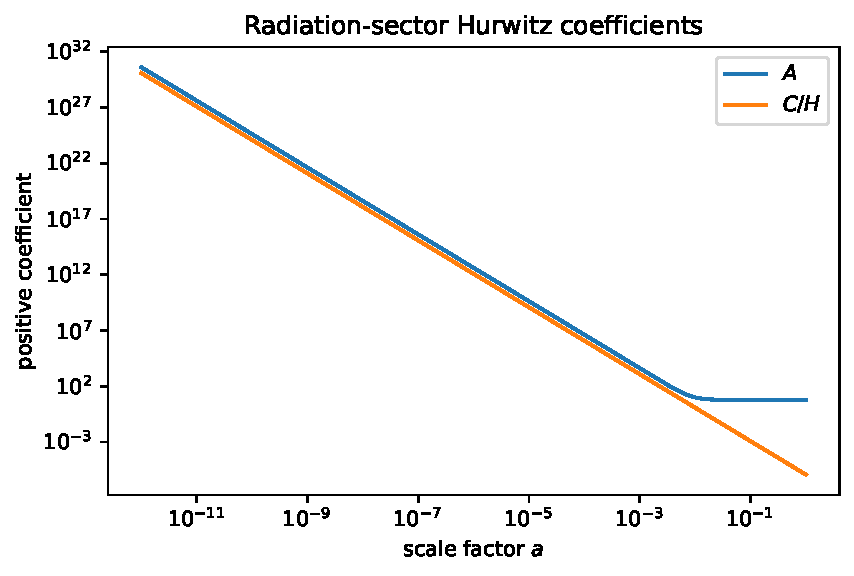
\includegraphics[width=\columnwidth]{figures/fig_radiation_stability.pdf}
\caption{Positive coefficients controlling the scalar radiation-sector Hurwitz polynomial along the tested background.}
\label{fig:hurwitz}
\end{figure}

\subsection{Matched operator-removal response}
At fixed homogeneous parameters and initial conditions, removing the mixed-current contribution produces a nonzero perturbative response. The maximum normalized differences are $0.3269$ internally, $0.3269$ in $E$, $0.2018$ in $\chi$, $7.11\times10^{-4}$ in $\delta$, and $9.87\times10^{-4}$ in $\theta$. The maximum relative differences in the tested CMB and linear matter spectra are $7.01\times10^{-3}$ and $2.18\times10^{-1}$, respectively. These values demonstrate that the operator has a causal perturbation-level role while leaving the homogeneous expansion unchanged.

\begin{figure}[htbp]
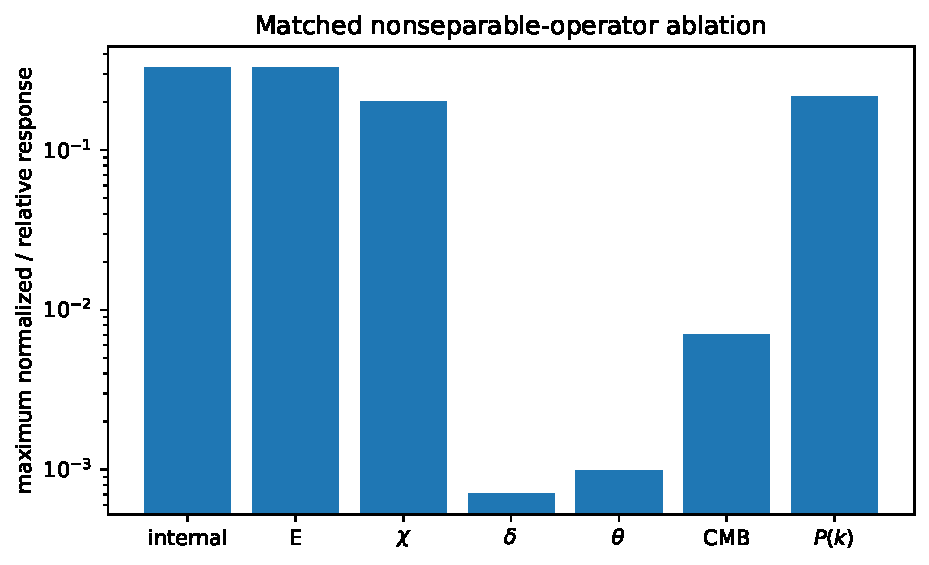
\includegraphics[width=\columnwidth]{figures/fig_operator_ablation.pdf}
\caption{Matched operator-removal response. The homogeneous background, initial conditions, and numerical settings are fixed while the nonseparable direct scalar contribution is removed in the control calculation.}
\label{fig:ablation}
\end{figure}

\subsection{Degrees of freedom and effective-field-theory scale}
The analyzed nonlinear phase space has dimension 42, with six first-class and eighteen second-class constraints, giving
\begin{equation}
N_{\rm dof}=\frac{42-2(6)-18}{2}=6.
\end{equation}
The auxiliary acceleration sector introduces no additional propagating scalar after its constraints are eliminated, while the nonseparable scalar operator changes neither the number of configuration variables nor the highest time-derivative order.

Including the temporal, mixed, and MOND cubic vertices, the canonically normalized propagating scalar has
\begin{equation}
\Lambda_{\rm sc,min}=1.47423693\times10^{-6}\ {\rm eV}
\end{equation}
at $a=6.44196\times10^{-3}$, where the mixed vertex controls the minimum. The minimum ratio of this scale to the tested reference expansion scale exceeds $1.7\times10^{10}$.

The companion scalar is first order. After solving its second-class constraints,
\begin{equation}
\Theta_{\rm red}=p_\chi d\chi-\Delta_k\Phi\,du,
\end{equation}
with
\begin{equation}
\Delta_k=ak^2+\frac32I_0\Q
\end{equation}
in the conservative matter-free case and an additional positive $\frac32a^3\rho_m$ term with matter. The tested minimum is $6.0136920\times10^{-8}\,\mathrm{Mpc}^{-2}$ and $\Delta_k^{-1}\sim k^{-2}$ at high $k$, so the constraint reduction is infrared finite and ultraviolet soft.

\subsection{Final cosmological likelihood}
Table~\ref{tab:likes} gives the independently replayed likelihood contributions. Their sum is
\begin{equation}
\chi^2_{\rm MG}=2422.695966726233.
\end{equation}
The matched optimized $\LCDM$ reference has $\chi^2=2428.9192$, so
\begin{equation}
\Delta\chi^2_{\rm MG-\LCDM}=-6.2232333.
\end{equation}
For seven fitted coordinates in the modified-gravity realization and six in the reference model, using the matched-analysis convention $N=2392$ for BIC,
\begin{align}
\Delta\mathrm{AIC}_{\rm MG-\LCDM}&=-4.2232333,\\
\Delta\mathrm{BIC}_{\rm MG-\LCDM}&=+1.5566518.
\end{align}
Thus the maximum likelihood and AIC favor the modified-gravity realization in this matched comparison, whereas BIC gives a small preference to the lower-dimensional $\LCDM$ reference. Because the models are not being treated here as a one-parameter nested hypothesis test, we do not assign a Gaussian significance by taking $\sqrt{|\Delta\chi^2|}$.

\begin{table}[htbp]
\caption{Independent fresh likelihood evaluation at the final optimized point.}\label{tab:likes}
\begin{ruledtabular}
\begin{tabular}{lr}
Likelihood & $\chi^2$\\\hline
Planck high-$\ell$ TTTEEE-lite & 582.162661\\
Planck low-$\ell$ TT & 22.975009\\
Planck low-$\ell$ EE & 395.918446\\
Planck lensing & 8.967854\\
DESI DR2 BAO & 8.640020\\
Pantheon+ & 1404.031978\\\hline
Total & 2422.695967\\
\end{tabular}
\end{ruledtabular}
\end{table}

\begin{figure}[htbp]
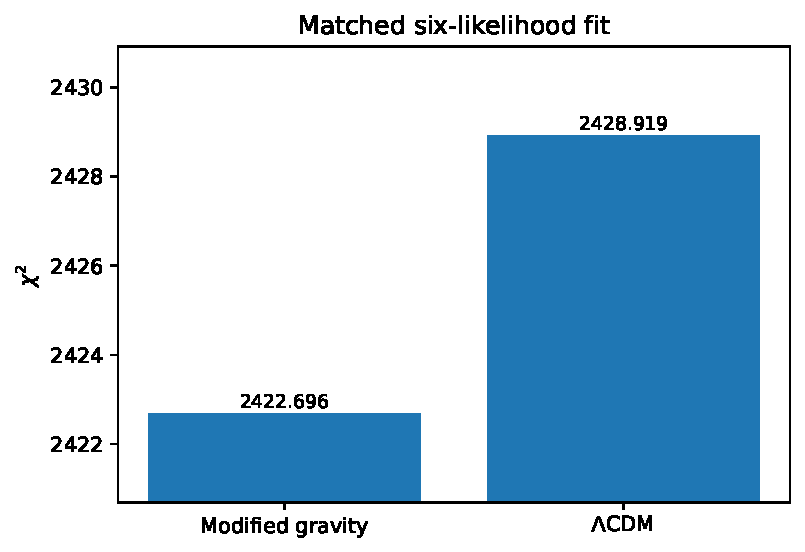
\includegraphics[width=\columnwidth]{figures/fig_chi2_comparison.pdf}
\caption{Total six-likelihood $\chi^2$ for the final modified-gravity realization and the matched optimized $\LCDM$ reference.}
\label{fig:chi2}
\end{figure}

\begin{figure}[htbp]
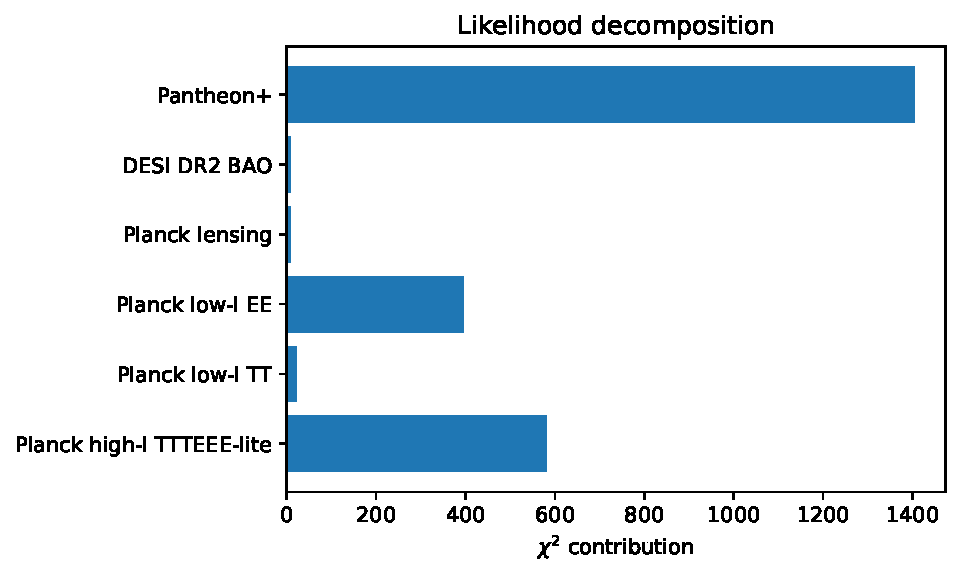
\includegraphics[width=\columnwidth]{figures/fig_likelihood_components.pdf}
\caption{Individual contributions to the final modified-gravity likelihood total.}
\label{fig:components}
\end{figure}

\subsection{Particle-CDM profile}
The independent profile has its lowest sampled value at $\omega_{\rm cdm}=0.001$. The exact zero-CDM point lies only
\begin{equation}
\Delta\chi^2(\omega_{\rm cdm}=0)=0.9581186
\end{equation}
above that sampled minimum. Thus the zero-particle-CDM realization is within $\Delta\chi^2<1$ of the profiled minimum. Across the tested grid the effective AeST cold density readjusts as explicit particle CDM is introduced. The appropriate conclusion is therefore that these data do not require nonzero particle CDM; they do not uniquely select exactly zero particle CDM.

\begin{figure}[htbp]
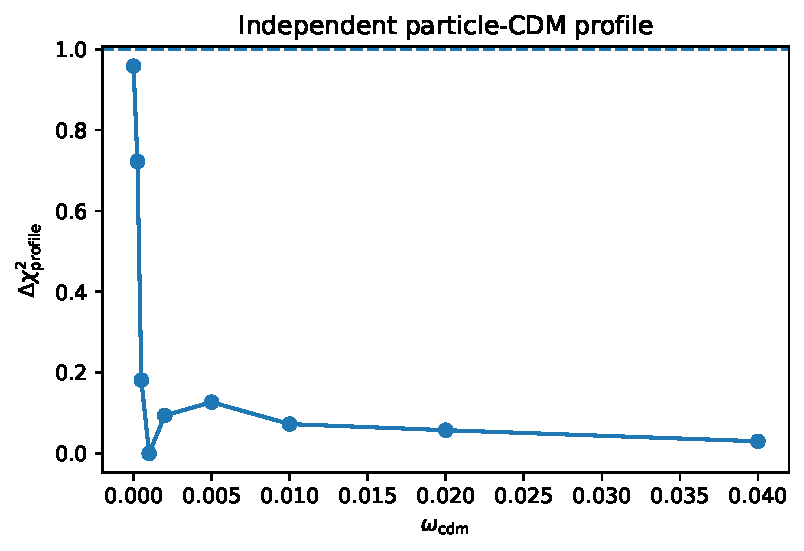
\includegraphics[width=\columnwidth]{figures/fig_cdm_profile.pdf}
\caption{Independent particle-CDM profile after reoptimization of the effective cold and cosmological coordinates at each sampled $\omega_{\rm cdm}$.}
\label{fig:profile}
\end{figure}

\subsection{Static galactic test}
In the screened static configuration $\Q=\Q_0$, so $\Gamma(\Q_0)=0$. The same $J(\Y)$ function therefore governs the static galaxy calculation. On the retained 132-galaxy, 2654-point SPARC subset, the baryons-only RMS scatter is $0.5121$ dex and the modified-gravity interpolation gives $0.1312$ dex, with no per-galaxy particle-dark-matter halo parameters. This result is not refitted by the cosmological nonseparable operator; rather, the operator is constructed to leave the tested static limit unchanged.

\section{Discussion}\label{sec:discussion}
The main structural result is a separation of physical roles. The timelike scalar sector provides an effective cold cosmological component, the noncanonical spatial scalar function provides the tested quasistatic MOND response, the nonseparable current-linked operator fixes the radiation-era scalar damping, and the auxiliary Type-II constraint sector supplies the reconstructed late-time acceleration. The new operator is therefore not an extra phenomenological function used to chase the cosmological likelihood; it is fixed by the conserved scalar current and accepted on stability grounds before the final cosmological optimization.

The statistical comparison should be interpreted conservatively. A lower $\chi^2$ and lower AIC show that the zero-particle-CDM realization is competitive with the matched $\LCDM$ reference within the chosen likelihood stack, while the small positive $\Delta$BIC reflects the larger parameter penalty in the adopted effective-$N$ convention. Neither statistic is a Bayes factor. Likewise, the particle-CDM profile shows that zero particle CDM is not disfavored at the $\Delta\chi^2=1$ level in the sampled profile, but the profile minimum is not exactly at zero. The data therefore support a non-requirement statement, not a detection of the absence of particle dark matter.

The effective-field-theory result is similarly scoped. Canonical normalization places the lowest tested cubic derivative scale many orders of magnitude above the cosmological frequencies and momenta used in the calculation, and the first-order scalar has a regular Dirac reduction. This establishes perturbative control over the tested classical domain. It is not a proof of a fundamental ultraviolet completion.

Several limitations remain relevant for future empirical tests. First, the cosmological analysis is linear; nonlinear large-scale structure, weak lensing, cluster mergers, and void statistics require a dedicated nonlinear solver. Second, the preferred-frame expressions reported in Appendix~\ref{app:dirac} are a screened limiting specialization; a complete moving-source finite-field 1PN derivation remains outside the present analysis. Third, the galactic calculation demonstrates the static no-halo limit on the retained SPARC sample, but cluster-scale morphology and environmental effects require separate analysis. These limitations are intentionally not hidden behind the successful linear-cosmology fit.

The combined construction also differs conceptually from adding a dark-energy fluid to AeST. The VCDM acceleration variable is auxiliary and does not supply another local propagating scalar mode \cite{DeFeliceMaedaMukohyamaPookkillath2022}. Conversely, the effective cold cosmological component is carried by the scalar--vector sector rather than by particle CDM. The final model thus separates the two conventional dark-sector roles into constrained gravitational dynamics rather than replacing both with a single invisible material component.

\section{Conclusions}\label{sec:conclusion}
We have constructed a single-metric relativistic modified-gravity cosmology combining an AeST scalar--vector sector with an auxiliary Type-II acceleration sector, while fixing particle cold dark matter and the bare cosmological constant to zero. The scalar kinetic function contains a current-linked nonseparable operator that leaves both the homogeneous scalar background and screened static galactic function unchanged but makes the radiation-era scalar system strictly damped on the physical branch. The same construction has a closed perturbation map in CLASS, a consistent nonlinear constraint count, a canonically controlled cubic scalar sector, and a regular first-order Dirac reduction.

After the theory source was fixed, the final Planck 2018 + DESI DR2 + Pantheon+ likelihood evaluation gave $\chi^2=2422.69597$, lower by $6.2232$ than the matched optimized $\LCDM$ reference. The corresponding AIC difference favors the modified-gravity realization, whereas the adopted BIC convention slightly favors the lower-dimensional reference. An independent particle-CDM profile places the exact zero-CDM realization within $\Delta\chi^2<1$ of its sampled minimum. The result therefore establishes a stable and observationally competitive zero-particle-CDM realization, while stopping short of claiming that current data uniquely require the absence of particle dark matter.

The source code, exact parameter file, numerical summaries, figure-generation scripts, and reproducibility hashes are prepared for public release so that each principal result can be independently retested.


\begin{acknowledgments}
The author declares no institutional affiliation and no specific external funding for this work. Public Planck, DESI, Pantheon+, SPARC, CLASS, and Cobaya resources were used as cited in the text.
\end{acknowledgments}

\section*{Artificial-intelligence assistance disclosure}
Substantive artificial-intelligence assistance was provided by OpenAI ChatGPT (GPT-5.6 Sol) and Google Antigravity using Gemini 3.7 Flash (High reasoning) for algebraic cross-checking, code generation and debugging, workflow organization, literature organization, and manuscript language editing. All executable calculations reported in this article were run in the author's computing environment. The author reviewed the equations, source changes, numerical outputs, citations, and scientific claims and assumes full responsibility for the accuracy and integrity of the work.

\section*{Data Availability Statement}
The observational data used in this work are publicly available through the Planck, DESI, Pantheon+, and SPARC releases cited in this article. The modified CLASS source, exact optimized parameter file, analysis and validation scripts, figure-generation code, machine-readable likelihood summaries, and cryptographic reproducibility manifests are prepared for release at \url{https://github.com/KarmirisP/aest-nonseparable-cosmology}. The exact submitted release will also be deposited in a DOI-bearing archival repository; the DOI will be inserted here before final submission.

\appendix
\section{Action, conventions, and scalar derivatives}\label{app:action}
We use metric signature $(-,+,+,+)$ and the definitions of Sec.~\ref{sec:theory}. The scalar--vector action is Eq.~\eqref{eq:aest-action}, with the nonseparable function Eq.~\eqref{eq:fullF}. On the homogeneous branch $\Y=0$,
\begin{align}
F_{,\Y}&=\Gamma(\Q),\\
F_{,\Y\Q}&=\Gamma_{,\Q},\\
F_{,\Q}&=\mathcal F_{T,\Q},\\
F_{,\Q\Q}&=\mathcal F_{T,\Q\Q}.
\end{align}
At the static screened point $\Q=\Q_0$,
\begin{equation}
\Gamma(\Q_0)=0,
\end{equation}
while $F_{,\Y\Q}$ need not vanish. Since $\Y$ is quadratic in spatial scalar gradients, the first nonzero mixed $F_{,\Y\Q}$ contribution is cubic in perturbations, explaining why the new coefficient enters the cubic cutoff calculation but not as an independent direct quadratic source.

For completeness, varying the Type-II auxiliary multiplier in Eq.~\eqref{eq:vcdm-aux} gives
\begin{equation}
-\frac32\lambda_C-(K+\varphi_V)=0,
\end{equation}
which yields the reduced term Eq.~\eqref{eq:vcdm-red}. In the scalar perturbation sector at nonzero wavenumber, the auxiliary equations set $\delta\varphi_V=0$ and fix the associated multipliers algebraically. Thus the acceleration sector alters the constraint equations and background reconstruction without adding a local scalar oscillator. This is the same degree-of-freedom property that characterizes VCDM in the Type-II minimally modified gravity literature \cite{DeFeliceMaedaMukohyamaPookkillath2022,GanzMartensMukohyamaNamba2023}.

The full scalar Euler--Lagrange equation follows from the shift symmetry. Writing the scalar contribution as $\sqrt{-g}\,L(\nabla\phi,A,g)$, it takes current-conservation form $\nabla_\mu \mathcal J^\mu_\phi=0$, where the timelike projection contains $F_{,\Q}$ and the projected spatial part contains $F_{,\Y}q^{\mu\nu}\nabla_\nu\phi$. In FLRW the spatial contribution vanishes identically, leaving the conserved quantity derived in Appendix~\ref{app:flrw}. This derivation is also the reason $\Gamma(\Q)$ cannot be adjusted independently once the current solution and temporal function are fixed.

\section{FLRW reduction and conserved current}\label{app:flrw}
For a spatially homogeneous scalar, $\Y=0$. The shift-symmetric scalar equation integrates once to
\begin{equation}
I_0=a^3\Q F_{,\Y}.
\label{eq:current}
\end{equation}
For Eq.~\eqref{eq:fullF},
\begin{equation}
I_0=2K_2Z_0a^3\sinh\left(\frac{\Q-\Q_0}{Z_0}\right).
\end{equation}
Defining $x_0\equiv I_0/(2K_2Z_0)$ yields the exact solution
\begin{equation}
\Q(a)=\Q_0+Z_0\operatorname{asinh}\left(\frac{x_0}{a^3}\right),
\label{eq:Qa}
\end{equation}
and hence
\begin{equation}
I_0=2K_2Z_0x_0.
\end{equation}
The final implementation uses $K_2=7500$, $\Q_0=0.1$, $Z_0=10^{-9}$, $x_0=0.02672752$, and $I_0=4.009128\times10^{-7}$ in the solver convention.

Because $\Y=0$ exactly, adding $\Y\Gamma(\Q)$ does not alter $\FT$, $\mathcal F_{T,\Q}$, or $\mathcal F_{T,\Q\Q}$ on FLRW. Numerical matched-background calculations confirmed equality to machine precision when only the mixed operator was removed. The late-time expansion sector is separately reconstructed through the auxiliary constraint potential, with flat closure recomputed from Eq.~\eqref{eq:vcdm-closure} at each likelihood point.

A key numerical detail is that the identity $K_Q-\Q F_{,\Y}=0$ should not be formed by subtracting two large nearly equal floating-point quantities at small $a$. The final implementation imposes the analytic cancellation directly and audits Eq.~\eqref{eq:current} independently.

\section{Linear scalar perturbations and CLASS variable map}\label{app:linear}
The quadratic derivation is organized so that the physical CLASS scalar combination is exposed before implementation. In the notation used during the variation,
\begin{equation}
\theta_s=\frac{\varphi}{\Q},\qquad
\alpha=\frac{\chi}{\Q}-\theta_s,
\end{equation}
so
\begin{equation}
\varphi+\Q\alpha=\chi.
\end{equation}
The quadratic contribution from the nonseparable operator therefore reduces to
\begin{equation}
\Delta\mathcal L^{(2)}=-\Gamma(\Q)\frac{k^2}{a^2}\chi^2
\end{equation}
in the physical scalar basis.

The generic direct source entering the $E$ equation contains
\begin{equation}
K_Q\chi-\Q F_{,\Y}\chi-(2-K_B)B.
\end{equation}
The current identity gives
\begin{equation}
K_Q=\Q F_{,\Y}=\frac{I_0}{a^3},
\end{equation}
so the direct $\chi$ source cancels exactly and the corresponding reduced equation contains
\begin{equation}
K_B(\dot E+HE)=-(2-K_B)B
\end{equation}
for this direct source contribution. The numerical source therefore inserts an analytic zero rather than a floating-point subtraction.

The mixed derivative $F_{,\Y\Q}=\Gamma_{,\Q}$ first contributes at cubic order. The kinematic definitions of the AeST density, velocity, $\chi$, anisotropic stress, and composite perturbation variables are unchanged by the nonseparable operator. In the auxiliary acceleration sector, the nonzero-$k$ scalar perturbations of the auxiliary field and gauge-fixing variables are eliminated algebraically, so the physical propagating scalar basis remains that of the scalar--vector gravitational sector after the metric constraints are solved.

\section{Constraint algebra and degree-of-freedom count}\label{app:dirac}
The background-independent combined analysis uses a 42-dimensional phase space and a 24-constraint system. Six constraints are first class and eighteen are second class, giving
\begin{equation}
N_{\rm dof}=\frac{42-2N_{\rm FC}-N_{\rm SC}}{2}
=\frac{42-12-18}{2}=6.
\end{equation}
The second-class submatrix was verified to have rank 18 on deterministic generic algebraic patches, while the expected first-class null directions were identified separately. The nonseparable scalar operator adds neither a configuration variable nor higher time derivatives, and the VCDM auxiliary variables are removed by second-class/algebraic constraints rather than becoming an extra propagating scalar. The AeST part of this count is consistent with the independent fully nonlinear Hamiltonian analysis of Bataki, Skordis, and Zlosnik \cite{BatakiSkordisZlosnik2024}; the absence of an extra local scalar in VCDM is consistent with the Type-II minimally modified gravity analysis \cite{DeFeliceMaedaMukohyamaPookkillath2022}.

For local preferred-frame behavior we quote only the screened Einstein--aether limiting specialization used as a structural check. In that limit,
\begin{equation}
\alpha_1=-4K_B^{\rm loc},
\end{equation}
\begin{equation}
\alpha_2=\frac{K_B^{\rm loc}[K_B^{\rm loc}-c_2(1-2K_B^{\rm loc})]}{c_2(2-K_B^{\rm loc})}.
\end{equation}
The relation $c_2=K_B^{\rm loc}/(1-2K_B^{\rm loc})$ with $K_B^{\rm loc}=10^{-5}$ gives $\alpha_1=-4\times10^{-5}$ and $\alpha_2=0$ in this screened limit \cite{FosterJacobson2006}. This appendix does not claim that the limiting formula replaces a complete moving-source finite-field 1PN calculation of the full theory.

\section{Canonical cubic scale and first-order symplectic reduction}\label{app:cutoff}
\subsection{Propagating scalar}
The quadratic principal scalar action defines a canonical field normalization proportional to $\mpl\sqrt{Z/2}$, with
\begin{equation}
Z=4K_2\cosh[(\Q-\Q_0)/Z_0].
\end{equation}
Three cubic channels are retained in the cutoff calculation: the temporal $F_{,\Q\Q\Q}$ vertex, the mixed $\Gamma_{,\Q}$ vertex, and the $\Y^{3/2}$ term in the MOND function. After canonical and acoustic-coordinate normalization, the instantaneous scales were scanned from $a=10^{-12}$ to $a=1$ using $10^5$ background samples. The minimum combined scale is
\begin{equation}
\Lambda_{\rm sc,min}=1.474236930936546\times10^{-6}\ {\rm eV},
\end{equation}
at $a=0.006441960984171227$, controlled by the mixed interaction. The same scan verifies the exact current identity and positive scalar sound speed.

The dimensionless regularity ratio
\begin{equation}
\left|\frac{\Q\Gamma_{,\Q}}{\mathcal{F}_{T,\Q\Q}}\right|<0.500000001
\end{equation}
over the tested branch demonstrates that the new mixed coefficient has no early-time parametric divergence relative to the temporal quadratic curvature, but this ratio is not itself the cutoff. The quoted energy scale follows from canonical normalization.

\subsection{First-order scalar}
The remaining scalar is described by a rank-two second-class pair. Solving the primary constraints gives
\begin{equation}
\Theta_{\rm red}=p_\chi d\chi-\Delta_k\Phi\,du,
\end{equation}
so the two scalar canonical pairs are $(\chi,p_\chi)$ and $(u,P_s)$ with
\begin{equation}
P_s=-\Delta_k\Phi.
\end{equation}
The conservative matter-free bracket is
\begin{equation}
\Delta_k=ak^2+\frac32I_0\Q,
\end{equation}
and matter contributes $+(3/2)a^3\rho_m$. Its $2\times2$ antisymmetric Dirac block has condition number one whenever $\Delta_k\neq0$. At $k=0$, $I_0>0$ and $\Q>0$ ensure strict positivity; at large $k$,
\begin{equation}
\Delta_k^{-1}\sim\frac{1}{ak^2}.
\end{equation}
Thus the reduction is infrared finite and ultraviolet soft. No separate second-order kinetic cutoff is assigned to this first-order canonical mode, and no fundamental quantum ultraviolet completion is inferred.

\section{CLASS implementation and numerical regression}\label{app:class}
The publication source is identified by the SHA-256 of \texttt{source/perturbations.c},
\begin{verbatim}
1b76e97333efd654736519bf324976dba
0906192f674f6d05e74f883f416c479
\end{verbatim}
The mixed-current helper quantities are evaluated from the exact background solution. In pseudocode,
\begin{verbatim}
x  = x0/a^3
FY = 2*K2*Z0*x/Q
QFY = 2*K2*Z0*x
\end{verbatim}
and the direct $(K_Q-\Q F_{,\Y})\chi$ contribution is set to analytic zero after an independent current-identity audit.

The implementation tests require: (i) successful clean builds; (ii) exact homogeneous background equality when the mixed operator alone is removed; (iii) finite CMB and matter spectra; (iv) source-diff locality; and (v) a nonzero physical spectral response to the matched operator-removal test. Radiation-era histories for $E_{\rm aest}$, $\chi_{\rm aest}$, $\delta_{\rm aest}$, and $\theta_{\rm aest}$ were checked across twelve histories and eight expected horizon crossings. Supported transfer outputs at redshifts $0,1,10,100,1000$ were finite and bounded. The claim does not extend high-redshift total-matter transfer certification beyond the gauge-invariant outputs actually exposed by the solver interface.

The public repository preserves the source tree byte-for-byte so the hash above can be checked independently. Development-era comments inside the frozen source may contain historical local labels; these comments are not scientific nomenclature and are intentionally not edited after the source freeze because doing so would destroy byte-level reproducibility.

\section{Likelihood implementation, optimization, and information criteria}\label{app:likelihood}
The final likelihood stack was evaluated with a frozen Python environment using NumPy 1.26.4, Cobaya \cite{TorradoLewis2021}, and the same external likelihood package directory for all matched comparisons. The likelihoods were Planck 2018 high-$\ell$ TTTEEE-lite, low-$\ell$ TT, low-$\ell$ EE, Planck lensing, DESI DR2 BAO, and Pantheon+.

The seven-dimensional fit varied $H_0$, $\omega_b$, $\omega_{\rm aest}$, $s_4$, $n_s$, $\ln(10^{10}A_s)$, and $\tau_{\rm reio}$. The scalar kinetic parameters were fixed before the fit, and $\omega_{\rm cdm}=\Omega_\Lambda=\Omega_{\rm fld}=0$ was enforced exactly. The dependent acceleration-basis coefficient and flat closure density were recomputed at every trial point.

The final optimized coordinates are
\begin{align}
H_0&=68.3206477851\ \mathrm{km\,s^{-1}\,Mpc^{-1}},\\
\omega_b&=0.02243860420,\\
\omega_{\rm aest}&=0.11881381554,\\
s_4&=0.34388729988,\\
n_s&=0.96752297007,\\
\ln(10^{10}A_s)&=3.03980058719,\\
\tau_{\rm reio}&=0.05408116437.
\end{align}
The corresponding $A_s=2.090107487735015\times10^{-9}$, $\Omega_V=0.6972944613049423$, and dependent coefficient $s_3=1.891402037916349$.

The initial scaled Nelder--Mead search reached its function-evaluation ceiling after locating a stable best point. Convergence was therefore certified independently: the exact best INI was replayed byte-for-byte; multiple evaluator labels gave identical totals; the point was polished with smaller deterministic coordinate steps; a fresh replay was identical at the reported numerical precision; and symmetric final displacements found no material downhill coordinate direction within the stated tolerance.

The information criteria are
\begin{equation}
\mathrm{AIC}=\chi^2+2k,\qquad
\mathrm{BIC}=\chi^2+k\ln N.
\end{equation}
We use $k_{\rm MG}=7$, $k_{\LCDM}=6$, and the matched-analysis convention $N=2392$. Because the likelihood is a combination of correlated data products, this $N$ is explicitly stated rather than presented as a unique universal definition of an effective BIC sample size \cite{Liddle2007}.

\section{Reproducibility and public release}\label{app:repro}
The publication source is anchored by cryptographic hashes. The final perturbation-source SHA-256 is
\begin{verbatim}
1b76e97333efd654736519bf324976dba
0906192f674f6d05e74f883f416c479
\end{verbatim}
The exact optimized parameter file, machine-readable likelihood table, particle-CDM profile summary, static-galaxy summary, figure input JSON, build environment, and regression scripts are included in the public release manifest.

The repository is organized as a testable publication product rather than a dump of exploratory working directories. It contains the exact modified CLASS tree, final parameter configuration, analysis scripts, compact publication evidence, tests, figures, manuscript source, and a SHA-256 release manifest. Larger source-of-truth research archives may be deposited as supplementary provenance in the DOI-bearing archival release without making the primary GitHub repository impractical to clone.

The public code repository is planned at
\begin{center}
\url{https://github.com/KarmirisP/aest-nonseparable-cosmology}.
\end{center}
The exact manuscript-submission tag should be archived in Zenodo or an equivalent DOI-bearing service. The DOI must be inserted into the Data Availability Statement and software citation before final submission. Upstream CLASS licensing and attribution must be retained for every redistributed CLASS-derived file.


\bibliography{references}
\end{document}
